% --------------------------------------------------------------
%                       Initialize
% --------------------------------------------------------------

\documentclass[11pt]{article}

% \usepackage{multicol}
\usepackage{ulem}
\usepackage{comment}
\newcommand{\todo}[1]{\textsc{{\color{red}#1}}}


\usepackage{personalNotes}
% contains special macros for math environment:
%     unit, p, set, abs, floor, ceil, vec, norm, inner, kernel
% contains useful all-purpose macros:
%     n, lessSeparation, append

\usepackage{tikz}
\usetikzlibrary{shapes,snakes}
\newcommand{\tedge}[5]{\draw[#3] (#1)-- node[e, #5] (e#4) {#4} (#2)}

% --------------------------------------------------------------
%                    Beginning of Document
% --------------------------------------------------------------

\begin{document}
% \begin{multicols}{2}

% --------------------------------------------------------------
%                           Title
% --------------------------------------------------------------

\pntitle {Decomposition Recombination Plans for 2D Well-Constrained Graphs}
\pnauthor{Troy Baker}
\pndate  {May 13, 2014}


\pnmaketitle
\pnmakefooter


% --------------------------------------------------------------
%                           Body
% --------------------------------------------------------------

\section{Introduction}
\todo{
Other sections...
\begin{itemize}
    \item Intro and motivation (previous work, where this work leads, examples)
    \item Preliminaries
    \item DR-Plan (Canonical) + algo
    \item Recombination + algo (refer to other paper and make 2D)
    \item Solution space navigation
    \item Conclusion
\end{itemize}
}

%%%%%%%%%%%%%%%%%%%%%%%%%%%%%%%%%%%%%%%%%%%%%%%%%%%%%%%%%%%%%%%%
%%%%%%%%%%%%%%%%%%%%%%%%%%%%%%%%%%%%%%%%%%%%%%%%%%%%%%%%%%%%%%%%
%%%%%%%%%%%%%%%%%%%%%%%%%%%%%%%%%%%%%%%%%%%%%%%%%%%%%%%%%%%%%%%%

\section{Preliminaries}



\subsection{Definitions}
% ISSUE: My definitions don't prevent non-positive densities... This means things aren't guaranteed to be connected...

\begin{definition}[Graph]
Graph $G=(V,E,w_V,w_E)$ is a set of vertices, $V$, and a set of edges, $E$, defined as a tuple of vertices from $V$. Additionally, there are two weight functions, $w_V: V \to \mathbb{R}^+$ and $w_E: E \to \mathbb{R}^+$.
\end{definition}

\begin{definition}[Density]
The density of a graph is defined as:
\[d(G) = \sum_{e\in E}{w_E(e)} - \sum_{v\in V}{w_V(v)}\]
% \[d(G) = \max\set{0,\sum_{v\in V}{w_V(v)} - \sum_{e\in E}{w_E(e)}}\]
\end{definition}

\begin{definition}[Independent or Sparse Graph]
\todo{Needs definition.}
\end{definition}

\begin{definition}[Over-constrained Graph]
Graph $G=(V,E,w_V,w_E)$ is over-constrained if, given constant $k$, there exists some induced subgraph $S\subseteq G$ such that $d(S) > k$. (where S is not trivial... This seems weird because you could have an over-constrained under-constrained graph...)
\end{definition}

\begin{definition}[Well-constrained Graph]
Graph $G=(V,E,w_V,w_E)$ is well-constrained if, given constant $k$, $d(G) = k$ and for all induced subgraphs $S\subseteq G$, (1) $d(S)\leq k$, or (2) given a set of trivial graphs $T$, $S$ is isomorphic to one of the graphs in $T$ (i.e.\ $S$ is trivial).
\end{definition}

% \begin{definition}[Well-constrained Graph]
% Graph $G=(V,E,w_V,w_E)$ is well-constrained if, given constant $k$ and a set of trivial graphs $T$, the graph satisfies (1) $d(G)=k$ and (2) all subgraphs are either under-constrained, well-constrained, or trivial (i.e.\ are isomorphic to one of the graphs in $T$).
% \end{definition}

\begin{definition}[Rigid Graph]
Graph $G=(V,E,w_V,w_E)$ is rigid if, given constant $k$, there exists some spanning subgraph $S\subseteq G$ such that $S$ is well-constrained.
\end{definition}

\begin{definition}[Under-constrained Graph]
Graph $G=(V,E,w_V,w_E)$ is under-constrained if, given constant $k$, $G$ is not rigid.
\end{definition}

% \begin{definition}[Under-constrained Graph]
% Graph $G=(V,E,w_V,w_E)$ is under-constrained if, given constant $k$, there exists some subgraph $G'\subseteq G$ such that $d(G') < k$.
% \end{definition}

\begin{definition}[Trivial Graph]
A trivial graph is ill-defined in the general case. The only strict requirements are: (1) it must be an over-constrained graph and (2) all of its subgraphs are also trivial.

\todo{Maybe leave this out until it's needed later?}
In the familiar geometric cases of $d$-dimensional space, all vertex weights are $d$, all edge weights are $1$, and constant $k= -{{d+1}\choose{2}}$. Trivial graphs for 2D would be a single vertex. Trivial graphs in 3D would be a vertex and an edge (2 vertices with an edge between). Etc. These trivial graphs capture the notion of the rotational symmetry that exists in geometric spaces.
\end{definition}

\begin{definition}[Decomposition Recombination (DR-) Plan]
The DR-plan of graph $G$, $DRP(G)$, is defined as a tree that has the following properties:
\begin{enumerate}
    \item The root of the tree `contains' $G$.
    \item For all nodes, $C$, that `contain' nontrivial graphs, its $N$ children, $C_1, \ldots, C_N$, are trivial or well-constrained vertex-maximal proper subgraphs of that node $C$.
    \item The vertex set of $\bigcup_{i=1}^N{C_i}$ is the vertex set of $C$.
    \item A node with a trivial subgraph is a leaf.
\end{enumerate}
% It can also be described recursively as: the root is $G$, its children are the trivial subgraphs and the DR-plans of its well-constrained vertex-maximal proper subgraphs whose union is $G$ itself.

An equivalent DAG can be constructed from this tree such that all nodes containing the same subgraphs are combined into one, with all edges preserved.

Note that nodes will be referred to interchangeably as ``the node that contains the (sub)graph $C$'' and as simply ``$C$''.
\end{definition}

\begin{definition}[Complete DR-Plan]
The complete DR-plan of graph $G$, $CompleteDRP(G)$, is the unique DR-plan but with a modified rule number 2: the children are \textit{all} of the trivial or well-constrained vertex-maximal proper subgraphs of that node $C$. By this, rule 3 is implicit for a complete DR-plan.
\end{definition}


\begin{definition}[Optimal DR-Plan]
The optimal DR-plan of graph $G$, $OptimalDRP(G)$, is the DR-plan that minimizes the maximum fan-in over all nodes in the tree. It is not necessarily unique.
\end{definition}


%%%%%%%%%%%%%%%%%%%%%%%%%%%%%%%%%%%%%%%%%%%%%%%%%%%%%%%%%%%%%%%%
%%%%%%%%%%%%%%%%%%%%%%%%%%%%%%%%%%%%%%%%%%%%%%%%%%%%%%%%%%%%%%%%
%%%%%%%%%%%%%%%%%%%%%%%%%%%%%%%%%%%%%%%%%%%%%%%%%%%%%%%%%%%%%%%%

\subsection{Notation}
$G$ is taken to be a graph with values $(V,E,w_V,w_E)$. To keep problems meaningful we assume that $G$ is connected, as the methods discussed are used to solve systems of equations to establish linkages. It is not useful to solve for two bodies simultaneously if there are no constraints between them. Furthermore, to limit the scope of the paper, $G$ will always be taken to be well-constrained.
% THIS MEANS NO EDGES MAY BE LEFT OUT, ALSO.

$Idc(G,X)$ is the graph induced on $G$ with the vertex set $X\subseteq V$. This can also be overloaded such that, using graph $H=(W,F)$, $Idc(G,H)=Idc(G,W)$.

$C$ is an arbitrary graph in a node in $CompleteDRP(G)$. $C_i$ is the $i^{\text{th}}$ child of $C$. By definition of a DR-plan, it is implied that $C_i$ is a well-constrained vertex-maximal proper subgraph.


%%%%%%%%%%%%%%%%%%%%%%%%%%%%%%%%%%%%%%%%%%%%%%%%%%%%%%%%%%%%%%%%
%%%%%%%%%%%%%%%%%%%%%%%%%%%%%%%%%%%%%%%%%%%%%%%%%%%%%%%%%%%%%%%%
%%%%%%%%%%%%%%%%%%%%%%%%%%%%%%%%%%%%%%%%%%%%%%%%%%%%%%%%%%%%%%%%

\section{The Canonical Optimal DR-Plan}
\begin{figure}
\begin{center}
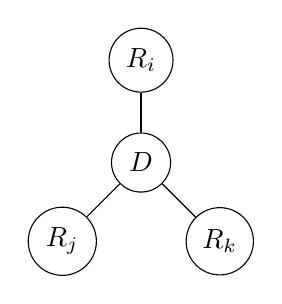
\begin{tikzpicture}
    \tikzstyle{v}=[draw, circle, minimum size=0.75cm]
    \tikzstyle{e}=[]

    \node[v] (v1) at (1,1) {$R_j$};
    \node[v] (v2) at (3,1) {$R_k$};
    \node[v] (v3) at (2,2) {$D$};
    \node[v] (v4) at (2,3.3) {$R_i$};

    \tedge{v1}{v3}{solid}{}{above};
    \tedge{v2}{v3}{solid}{}{above};
    \tedge{v3}{v4}{solid}{}{right};
\end{tikzpicture}
\ldots with weights \ldots
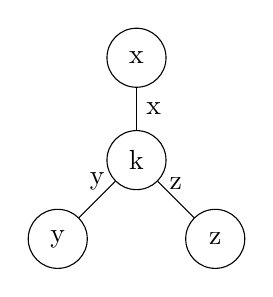
\begin{tikzpicture}
    \tikzstyle{v}=[draw, circle, minimum size=0.75cm]
    \tikzstyle{e}=[]

    \node[v] (v1) at (1,1) {y};
    \node[v] (v2) at (3,1) {z};
    \node[v] (v3) at (2,2) {k};
    \node[v] (v4) at (2,3.3) {x};

    \tedge{v1}{v3}{solid}{y}{above};
    \tedge{v2}{v3}{solid}{z}{above};
    \tedge{v3}{v4}{solid}{x}{right};

    % \draw (3.3,2.5) circle (1.9cm);
    % \draw (.7,2.5) circle (1.9cm);
    % \draw (2,.5) circle (1.9cm);
\end{tikzpicture}
\\
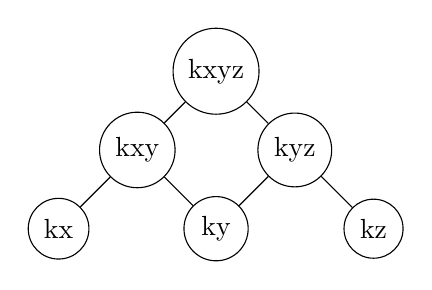
\begin{tikzpicture}
    \tikzstyle{v}=[draw, circle, minimum size=0.75cm]
    \tikzstyle{e}=[]

    \node[v] (v1) at (0,  0) {kxyz};
    \node[v] (v2) at (-1,-1) {kxy};
    \node[v] (v3) at ( 1,-1) {kyz};
    \node[v] (v4) at (-2,-2) {kx};
    \node[v] (v5) at ( 0,-2) {ky};
    \node[v] (v6) at ( 2,-2) {kz};

    \tedge{v1}{v2}{solid}{}{};
    \tedge{v1}{v3}{solid}{}{};
    \tedge{v2}{v4}{solid}{}{};
    \tedge{v2}{v5}{solid}{}{};
    \tedge{v3}{v5}{solid}{}{};
    \tedge{v3}{v6}{solid}{}{};
\end{tikzpicture}
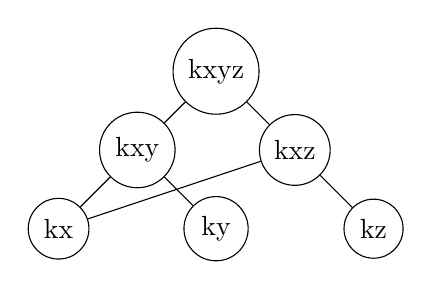
\begin{tikzpicture}
    \tikzstyle{v}=[draw, circle, minimum size=0.75cm]
    \tikzstyle{e}=[]

    \node[v] (v1) at (0,  0) {kxyz};
    \node[v] (v2) at (-1,-1) {kxy};
    \node[v] (v3) at ( 1,-1) {kxz};
    \node[v] (v4) at (-2,-2) {kx};
    \node[v] (v5) at ( 0,-2) {ky};
    \node[v] (v6) at ( 2,-2) {kz};

    \tedge{v1}{v2}{solid}{}{};
    \tedge{v1}{v3}{solid}{}{};
    \tedge{v2}{v4}{solid}{}{};
    \tedge{v2}{v5}{solid}{}{};
    \tedge{v3}{v4}{solid}{}{};
    \tedge{v3}{v6}{solid}{}{};
\end{tikzpicture}
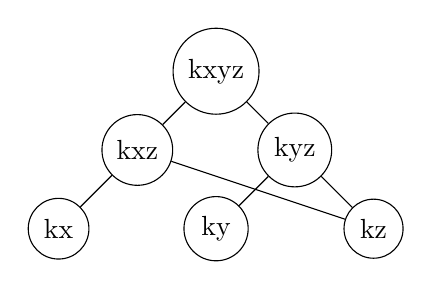
\begin{tikzpicture}
    \tikzstyle{v}=[draw, circle, minimum size=0.75cm]
    \tikzstyle{e}=[]

    \node[v] (v1) at (0,  0) {kxyz};
    \node[v] (v2) at (-1,-1) {kxz};
    \node[v] (v3) at ( 1,-1) {kyz};
    \node[v] (v4) at (-2,-2) {kx};
    \node[v] (v5) at ( 0,-2) {ky};
    \node[v] (v6) at ( 2,-2) {kz};

    \tedge{v1}{v2}{solid}{}{};
    \tedge{v1}{v3}{solid}{}{};
    \tedge{v2}{v4}{solid}{}{};
    \tedge{v2}{v6}{solid}{}{};
    \tedge{v3}{v5}{solid}{}{};
    \tedge{v3}{v6}{solid}{}{};
\end{tikzpicture}
% \\
% \begin{tikzpicture}
%     \tikzstyle{v}=[draw, circle, minimum size=0.75cm]
%     \tikzstyle{e}=[]

%     \node[v] (v1) at ( 0, 0) {kxyz};
%     \node[v] (v2) at (-1,-1) {kxy};
%     \node[v] (v3) at (-2,-2) {kx};
%     \node[v] (v4) at (-3,-3) {k};
%     \node[v] (v5) at ( 1,-1) {z plan};
%     \node[v] (v6) at ( 0,-2) {y plan};
%     \node[v] (v7) at (-1,-3) {x plan};
%     \node[v] (v8) at (-2,-4) {k plan};

%     \tedge{v1}{v2}{solid}{}{};
%     \tedge{v1}{v5}{solid}{}{};
%     \tedge{v2}{v3}{solid}{}{};
%     \tedge{v2}{v6}{solid}{}{};
%     \tedge{v3}{v4}{solid}{}{};
%     \tedge{v3}{v7}{solid}{}{};
%     \tedge{v4}{v8}{solid}{}{};
% \end{tikzpicture}
\end{center}

\caption{A well-constrained graph whose nodes are subgraphs labeled with their density. Below are its 3 optimal DR-Plans (partially complete). The center vertex has weight $k$ and is well-constrained itself. The radial nodes have weights $x,y,z \neq k$ with equivalent edge weights, making any union between $k$ and the others well-constrained. \todo{Make this figure more clear.}}
\label{3-plans}
\end{figure}

In the case of a well-constrained graph, it is clear that there always exists a unique vertex-maximum DR-Plan that includes every single well-constrained vertex-maximal proper subgraph at each node, which we call the complete DR-plan. However, in the problem of the optimal DR-Plan there is no such unique plan. For instance, a graph that is formed by the union of 3 well-constrained subgraphs that all intersect on a well-constrained subgraph, demonstrated in Figure \ref{3-plans}. In this case, it results in $3$ unique optimal DR-Plans. Indeed, we will prove a union of $N$ well-constrained subgraphs will result in $N$ unique plans, but that at the $N^{\text{th}}$ level of the tree it will always be the same. Therefore, all choices of decomposition are in some sense equivalent. The theorem we seek to prove is thus:

\begin{theorem}\label{t1}
Given a well-constrained 2-dimensional bar-joint graph $G$, for node $C$ in $OptimalDRP(G)$ and the children of $C$ in $CompleteDRP(C)$ labeled as $C_1,\ldots,C_N$
\begin{enumerate}
    \item if $C_i \cap C_j$ is trivial then all $C_1,\ldots,C_N$ are children of $C$ in $OptimalDRP(G)$
    \item if $C_i \cap C_j$ is well-constrained then any two out of $C_1,\ldots,C_N$ will be the only children of $C$ in $OptimalDRP(G)$.
\end{enumerate}
\end{theorem}

We develop this notion of the canonical optimal DR-plan by carefully considering the case of a union of any two nontrivial well-constrained vertex-maximal proper subgraphs of a well-constrained graph. By definition, any subgraph of a well-constrained graph will either be (1) trivial, (2) under-constrained, or (3) well-constrained. We will analyze all 3 possibilities in turn. These observations will lead to interesting properties that govern the behavior of optimal DR-plans on well-constrained graphs.

% We show this by carefully considering all of the potential cases of the unions of subgraphs. By definition, any subgraph of a well-constrained graph will either be (1) under-constrained, (2) well-constrained, or (3) trivial. We will analyze all 3 possibilities in turn, in the case of a union of any two nontrivial well-constrained vertex-maximal proper subgraphs.




%%%%%%%%%%%%%%%%%%%%%%%%%%%%%%%%%%%%%%%%%%%%%%%%%%%%%%%%%%%%%%%%
%%%%%%%%%%%%%%%%%%%%%%%%%%%%%%%%%%%%%%%%%%%%%%%%%%%%%%%%%%%%%%%%
%%%%%%%%%%%%%%%%%%%%%%%%%%%%%%%%%%%%%%%%%%%%%%%%%%%%%%%%%%%%%%%%

\subsection{Relationships for the Union and Intersection of Well-Constrained Subgraphs}
For the following lemmas, we define $F_i$ and $F_j$ as well-constrained subgraphs of the same well-constrained graph $F$.
We wish to prove the following bijections:

\begin{center}
\begin{tabular}{|c|c|}
\hline
\textbf{Union is\ldots} & \textbf{Intersection is\ldots} \\ \hline
\sout{trivial}          & --- \\ \hline
under-constrained       & trivial \\ \hline
well-constrained        & well-constrained \\ \hline
---                     & \sout{under-constrained} \\ \hline
\end{tabular}
\end{center}


\begin{lemma}\label{t-l1}
$F_i\cup F_j$ cannot be trivial.
\end{lemma}

\begin{proof}
% If $F_i,F_j$ are well-constrained, then $F_i\cup F_j \geq k$. Trivial graphs must be over-constrained.

Follows from the definition of a trivial graph. It would imply that the well-constrained graphs were also trivial since they would be subgraphs of a trivial graph.
\end{proof}


\begin{lemma}\label{uc-l1}
$F_i\cup F_j$ is under-constrained if and only if $F_i\cap F_j$ is trivial.
\end{lemma}

\begin{proof}
It follows from definitions that $d(F_i)=k$ and $d(F_j)=k$. In the forward direction, we have that $d(F_i\cup F_j)=l<k$. If it were equal to $k$ it would be well-constrained since, as a subgraph of $F$, it satisfies the other properties of a well-constrained graph; if it were greater than $k$ then it would be over-constrained. Therefore $d(F_i\cap F_j)=d(F_i)+d(F_j)-d(F_i\cup F_j)=2k-l>k$. The only way to have an over-constrained subgraph in a well-constrained graph is if it is trivial.

In the reverse direction, we know that $d(F_i\cap F_j)>k$ because it is trivial. Thus, by the same math, it is clear that $d(F_i\cup F_j)<k$ and it must be under-constrained.
\end{proof}


\begin{lemma}\label{wc-l1}
$F_i\cup F_j$ is well-constrained if and only if $F_i\cap F_j$ is well-constrained.
\end{lemma}

\begin{proof}
It follows from definitions that $d(F_i)=k$ and $d(F_j)=k$. In the forward direction we have that $d(F_i\cup F_j)=k$, therefore $d(F_i\cap F_j)=d(F_i)+d(F_j)-d(F_i\cup F_j)=k$. Since $F_i\cap F_j$ is a subgraph of $F$, which is well-constrained, it is also well-constrained.

In the reverse direction the same math proves that $d(F_i\cup F_j)=k$ and, since it is also a subgraph of $F$, it too is well-constrained.

% \todo{Integrate this}
% Furthermore, all subgraphs of $F_i\cup F_j$ and $F_i\cap F_j$ are also subgraphs of $F_i$ and $F_j$, therefore all properties of well-constrained graphs are maintained.

% In the forward direction: From Lemma \ref{uc-l1}, the intersection cannot be trivial. The intersection also cannot be under-constrained. If $F_i \cap F_j$ were under-constrained, then for $F_i$ to be well-constrained you would need to add more constraints (edge weight) than degrees of freedom (vertex weight) to the intersection. The same is true for $F_j$. If both of these were satisfied, then the union of $F_i$ and $F_j$ would result in an over-constrained nontrivial graph. This is a contradiction, by definition of a well-constrained graph. Therefore, the intersection can only be well-constrained.

% reverse!!!!!
\end{proof}


\begin{lemma}\label{iuc-l1}
$F_i\cap F_j$ cannot be under-constrained.
\end{lemma}

\begin{proof}
Subgraphs of well-constrained graph $F$ can only be trivial, under-constrained, or well-constrained. So it follows from Lemmas \ref{t-l1}, \ref{uc-l1}, and \ref{wc-l1} that only trivial and well-constrained intersections are possible.
\end{proof}

% WAIT... WHAT ABOUT TWO BANANAS? The intersection is 2 vertices which is under-constrained... oh nevermind... that's well-constrained




%%%%%%%%%%%%%%%%%%%%%%%%%%%%%%%%%%%%%%%%%%%%%%%%%%%%%%%%%%%%%%%%
%%%%%%%%%%%%%%%%%%%%%%%%%%%%%%%%%%%%%%%%%%%%%%%%%%%%%%%%%%%%%%%%
%%%%%%%%%%%%%%%%%%%%%%%%%%%%%%%%%%%%%%%%%%%%%%%%%%%%%%%%%%%%%%%%

\subsection{Inferring Graph Structure from Union and Intersection Properties}



\begin{lemma}\label{wc-l2}
% Given a well-constrained $G$ and two well-constrained vertex-maximal proper subgraphs $C_i, C_j$,
$C_i\cup C_j$ is well-constrained if and only if $C_i\cup C_j = C$.
\end{lemma}

\begin{proof}
The forwards direction can be shown with a contradiction. If the $C_i\cup C_j$ was well-constrained but $C_i\cup C_j \neq C$, we would have found a larger well-constrained proper subgraph containing them; namely, $C_i\cup C_j$ or something containing it would have been larger. The two original subgraphs could not have been vertex-maximal proper.

The reverse direction follows from the fact that $C$ is either some non-leaf node (well-constrained by definition of a DR-plan) or $G$ itself (well-constrained by definition of the problem).
\end{proof}

\begin{corollary}\label{wc-c1}
% Given a well-constrained $G$ and two well-constrained vertex-maximal proper subgraphs $C_i, C_j$, l
Let us say $R_i=C\setminus C_i$ and $R_j=C\setminus C_j$. If $C_i\cup C_j$ is well-constrained, then there can be no edges in $C$ between the vertices of $R_i$ and $R_j$.
\end{corollary}

\begin{proof}
It follows from the fact that $C_i\cup C_j$ must equal $C$ (proven in Lemma \ref{wc-l2}).
\end{proof}



At this point we limit our discussion to the scope of 2D graphs. All vertex weights are $2$, all edge weights are $1$, and constant $k= -{{3}\choose{2}}=-3$. Trivial graphs are a single vertex and empty set.

Also, 2D well-constrained graphs must be connected.
% \todo{Is this actually true?}
The greatest density of a 2D well-constrained graph is $-2$ (the vertex). The other disconnected part of the graph would need to have a density of $-1$, which is over-constrained and not possible in a well-constrained graph (because there is no trivial graph with that density).

\begin{lemma}\label{wc-l3}
If $C_i\cup C_j=C$, then $\forall k: C_i\cup C_k=C$.
Alternatively, if $C_i\cup C_j$ is well-constrained, then $\forall k: C_i\cup C_k$ is well-constrained.
\end{lemma}

\begin{proof}
Let us say $R_i=C\setminus C_i$, $R_j=C\setminus C_j$, and $D_{i,j}=C_i\cap C_j=(C\setminus R_i)\setminus R_j$ (note that $R_j\subset C_i$, $R_i\subset C_j$ and $D_{i,j}\subset C_i,C_j$). Furthermore, we have the proper subgraphs $R'_i\subset R_i$, $R'_j\subset R_j$, and $D'_{i,j}\subset D_{i,j}$ which are not empty sets.

Then we assume that there is some third well-constrained vertex-maximal proper subgraph $C_k$ (with $C'_k=C\setminus C_k$). There are $3\times 3\times 3 = 27$ possible cases for what this subgraph could be.

\begin{itemize}
    \item 3 cases: $C_k$ cannot be $C=Idc(C,R_i\cup R_j\cup D_{i,j})$, $C_i=Idc(C,R_j\cup D_{i,j})$, or $C_j=Idc(C,R_i\cup D_{i,j})$. This is by definition.

    \item 13 cases: $C_k$ cannot be a proper subgraph of $C_i$ and $C_j$ or else $C_k$ would not be vertex-maximal. These are the graphs $Idc(C,R'_i\cup D_{i,j})$, $Idc(C,R'_j\cup D_{i,j})$, $Idc(C, D_{i,j})$, $Idc(C,R_i\cup D'_{i,j})$, $Idc(C,R_j\cup D'_{i,j})$, $Idc(C,R'_i\cup D'_{i,j})$, $Idc(C,R'_j\cup D'_{i,j})$, $Idc(C, D'_{i,j})$, $Idc(C,R_i)$, $Idc(C,R_j)$, $Idc(C,R'_i)$, $Idc(C,R'_j)$, and $Idc(C,\emptyset)$.

    \item 2 cases: $C_k$ cannot contain $C_i$ or $C_j$ as proper subgraphs, or else they were not vertex-maximal. These are the graphs $Idc(C,R'_i\cup R_j\cup D_{i,j})$ and $Idc(C,R_i\cup R'_j\cup D_{i,j})$ respectively.

    \item 4 cases: \todo{Uses 2D requirement:} $C_k$ cannot be $Idc(C,R_i\cup R_j)$, $Idc(C,R'_i\cup R_j)$, $Idc(C,R_i\cup R'_j)$, or $Idc(C,R'_i\cup R'_j)$ because these are all disconnected (Corollary \ref{wc-c1}) and cannot be well-constrained.

    \item 1 case: $C_k=Idc(C,R'_i\cup R'_j\cup D_{i,j})$ is not possible. Since $C_k\cup C_i = Idc(C,R'_i\cup R_j\cup D_{i,j})\neq C$ we have from Lemma \ref{wc-l2} that $C_k\cup C_i$ cannot be well-constrained. We also know it cannot be trivial because it contains well-constrained subgraphs. This means it must be under-constrained. From Lemma \ref{uc-l1}, we know that $C_k\cap C_i=Idc(C,R'_j\cup D_{i,j})$ must then be trivial. This is impossible because $D_{i,j}$ is well-constrained, thereby contradicting the assumption that $C_k$ is well-constrained.

    \item 1 case: \todo{Uses 2D requirement:} $C_k=Idc(C,R'_i\cup R'_j\cup D'_{i,j})$ is not possible. The union with $C_i$ (or $C_j$) is not equal to $C$. Therefore, the union must be under-constrained which means the intersection must be trivial (a single node). However, $C_k\cap C_i=Idc(C,R'_j\cup D'_{i,j})$ and since $R'_j$ and $D'_{i,j}$ are not empty sets, it cannot be trivial making a contradiction.

    \item 2 cases: \todo{Uses 2D requirement:} $C_k=Idc(C,R'_i\cup R_j\cup D'_{i,j})$ and $C_k=Idc(C,R_i\cup R'_j\cup D'_{i,j})$ are not possible. The proof mirrors the previous case, except you must choose $C_i$ and $C_j$, respectively, here.

    \item 1 case: $C_k=Idc(C,R_i\cup R_j\cup D'_{i,j})$ is all that is left!
\end{itemize}

Since $D_{i,j}\subset C_i, C_j$ it means that $C_k\cup C_i = C_k \cup C_j = C$, thus proving the Lemma.

\todo{Needs a figure.}
\end{proof}



% \pnplaceholder
% WAIT, TRIVIAL GRAPH DEFINITION DOESN'T WORK!!!! in 4D it's the 3 clique, but 3 vertices is a subgraph of that... that is certainly not over-constrained...

% NOT SO! -5C2 = -10. 3 edges and 3 nodes -> 3 - 3*4 = -9... over-constrained!



% \pnplaceholder

\begin{lemma}\label{uc-l2}
% If there exist $C_i, C_j$ such that $C_i\cap C_j$ is trivial, then for all $C_k,C_l$, $C_k\cap C_l$ is trivial (a vertex or empty set).
If $C_i\cap C_j$ is trivial, then $\forall k: C_i\cap C_k$ is trivial.
\end{lemma}

\begin{proof}
If any intersection was not trivial, then it must be well-constrained. If $C_k\cap C_l$ were well-constrained, then by Lemma \ref{wc-l3} all of the intersections are well-constrained. This contradicts the statement that $C_i\cap C_j$ is trivial.
% It follows that if the intersection is trivial then the union is under-constrained (Lemma \ref{uc-l1}). If the union is under-constrained, then the
\end{proof}



%%%%%%%%%%%%%%%%%%%%%%%%%%%%%%%%%%%%%%%%%%%%%%%%%%%%%%%%%%%%%%%%
%%%%%%%%%%%%%%%%%%%%%%%%%%%%%%%%%%%%%%%%%%%%%%%%%%%%%%%%%%%%%%%%
%%%%%%%%%%%%%%%%%%%%%%%%%%%%%%%%%%%%%%%%%%%%%%%%%%%%%%%%%%%%%%%%


\subsection{Proving the Main Theorem}
Lemmas \ref{wc-l3} and \ref{uc-l2} show that $CompleteDRP(C)$ will result in one of two scenarios. (A) Either all $C_1,\ldots,C_N$ intersect on some common well-constrained subgraph and any two union to make $C$, or (B) all $C_1,\ldots,C_N$ intersect trivially and all of them must be unioned to make $C$.

% \begin{theorem}
% In case (A), any two unique wcvmps of $C$ can be used as the children of $C$ in $OptimalDRP(C)$.
% \end{theorem}

% \begin{proof}

% \end{proof}

% \begin{theorem}
% In case (B), all wcvmps of $C$ must be used as the children of $C$ in $OptimalDRP(C)$.
% \end{theorem}

% \begin{proof}
% If not all of them are used, the union will be under-constrained. $C$ is well-constrained, thus using not all of them is not an option.
% \end{proof}


% \pnplaceholder


% \pagebreak
% See ISSUE at top of paper, we have to assume we have a connected $G$...

% Take $C'_i$ to be $C\setminus C_i$. Then if $C_i\cup C_j$ is well-constrained we have directly from Lemma \ref{wc-l2} for all $C'_i, C'_j$ there can be no edges between them (otherwise $C_i\cup C_j\neq C$).

% The set of edges connecting $C'_i$ to $C_i$ must have a weight that sums to exactly $d(C'_i)$ since we know that $d(C)=d(C_i)=k$.

% Any other $C_k$ must therefore contain $C'_i$ and $C'_j$ because it adds no density to ``tack it on'' to a graph that does not contain them already.

% Now we want to know something about $C_k$. If $C_k \neq C_i$, then $C'_i\not\subseteq C'_k$. It is clear that they cannot be equal otherwise $C_k = C_i$. However, it also cannot be a subset. There are two scenarios. (1) $C'_k$ does not contain vertices that are incident to $C'_i$. If this were so, we know we could ``tack on'' $C'_i$ to the well-constrained $C_k$ without increasing the density and therefore $C_k$ could not have been maximal in the first place. (2) $C'_k$ contains vertices that are incident to $C'_i$. In this case

% Take $D_{i,j}$ to be $C\setminus (C'_i\cup C'_j)$. Clearly $D_{i,j}$ must be well-constrained since ``tacking on'' $C'_i$ and $C'_j$ adds no density and $C$ is well-constrained. Therefore, if there were some other $C_k$, it must contain $D_{i,j,k}\subset D_{i,j}$ such that $D_{i,j,k}=D_{i,j}\setminus C'_k$. It is clear that $D_{i,j,k}$ cannot equal $D_{i,j}$ or else $C_k$ must be $C_i$ or $C_j$ to be vertex-maximal.


% \begin{lemma}
% If there exist $C_i, C_j$ such that $C_i\cap C_j$ is trivial, then for all $C_k,C_l$, $C_k\cap C_l$ is trivial or empty set.
% \end{lemma}

% \begin{proof}
% By Lemmas... the union must be under
% Lemma \ref{uc-l1} that $C_i\cup C_j$ must be under-constrained. Therefore, by the proof
% It follows from Lemma \ref{wc-l1} that the only way to get
%  and its proof that if any intersections
% \end{proof}





\begin{figure}
\begin{center}
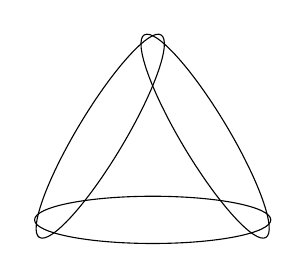
\begin{tikzpicture}
    \draw[rotate=0]  (0,0) ellipse (1.5cm and .3cm);
    \draw[rotate around={-59:(.7,1.2)}] (.8,1.1) ellipse (1.5cm and .3cm);
    \draw[rotate around={59:(-.7,1.2)}] (-.8,1.1) ellipse (1.5cm and .3cm);

    % \draw[rotate around={59:(.7,-1.2)}] (.8,-1.1) ellipse (1.5cm and .3cm);
    % \draw[rotate around={-59:(-.7,-1.2)}] (-.8,-1.1) ellipse (1.5cm and .3cm);

    % \draw[rotate=0] (1,1) ellipse (.1cm and .1cm);
    % \draw[rotate=66] (0,0) ellipse (.1cm and .1cm);
\end{tikzpicture}
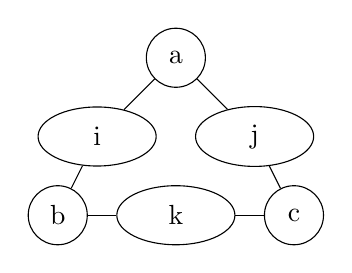
\begin{tikzpicture}
    \tikzstyle{v}=[draw, circle, minimum size=0.75cm]
    \tikzstyle{el}=[draw, ellipse, minimum height=.75cm, minimum width=1.5cm]
    \tikzstyle{e}=[]

    \node[el] (m) at (0,    0) {k};
    \node[v]  (l) at (-1.5, 0) {b};
    \node[v]  (r) at (1.5,  0) {c};

    \node[el] (tl) at (-1,  1) {i};
    \node[el] (tr) at (1,   1) {j};
    \node[v]  (t)  at (0,   2) {a};

    % \node[el] (bl) at (-1,  -1) {l};
    % \node[el] (br) at (1,   -1) {m};
    % \node[v]  (b)  at (0,   -2) {d};

    % \node[el] (v2) at (-1,-1) {b};
    % \node[el] (v3) at (-1,-1) {b};
    % \node[el] (v4) at (-1,-1) {b};
    % \node[el] (v5) at (-1,-1) {b};

    \tedge{m}{l}{solid}{}{};
    \tedge{m}{r}{solid}{}{};

    \tedge{l}{tl}{solid}{}{};
    \tedge{tl}{t}{solid}{}{};
    \tedge{r}{tr}{solid}{}{};
    \tedge{tr}{t}{solid}{}{};

    % \tedge{l}{bl}{solid}{}{};
    % \tedge{bl}{b}{solid}{}{};
    % \tedge{r}{br}{solid}{}{};
    % \tedge{br}{b}{solid}{}{};
\end{tikzpicture}
\end{center}

\caption{Each node contains a subgraph of the entire, well-constrained graph $G$. We take $Idc(G,a\cup i\cup b)$, $Idc(G,a\cup j\cup c)$, and $Idc(G,b\cup k\cup c)$ to be well-constrained. If the union of any two of these listed unions is under-constrained then it immediately follows that all such unions are under-constrained and that nodes $a,b,c$ must all be trivial subgraphs.
% Each node contains a subgraph of the entire, well-constrained graph. We take $a\cup i\cup b$, $a\cup j\cup c$, $b\cup k\cup c$, $b\cup l\cup d$, and $c\cup m\cup d$ to be well-constrained. If the union of any two of these listed unions is under-constrained then it immediately follows that all such unions are under-constrained and that nodes $a,b,c,d$ must all be trivial subgraphs.
% THIS IS NOT TECHNICALLY CORRECT... $a\cup i\cup b$ doesn't include the edge between them... Is there a better way to phrase this?
}
\label{trivial-intersection}
\end{figure}


\begin{theorem}\label{uc-t1}
% In any solution to $OptimalDRP(G)$, if any two well-constrained vertex-maximal proper subgraphs of a node form a union that is under-constrained, then all well-constrained vertex-maximal proper subgraphs of said node must be included in the optimal plan.

In $OptimalDRP(G)$ of a well-constrained $G$, if $C_i \cap C_j$ is trivial (case (B)), then all $C_1,\ldots, C_N$ must be included in the optimal plan as children of $C$.
\end{theorem}

\begin{proof}
From Lemma \ref{uc-l1}, if it is trivial then $C_i \cup C_j$ must be under-constrained. If it is under-constrained, it must be part of some larger well-constrained subgraph $D$. If $D$ is not $G$ itself, then we just found a larger proper subgraph and the graphs in the set were not vertex-maximal to begin with.
 % For $C$ to be well-constrained... WHAT????

If there was some $X\subset [1,\ldots,N]$ such that $\bigcup_{i\in X}{C_i}\neq C$ but it was well-constrained, then we just found a larger proper subgraph and the graphs in the set were not vertex-maximal to begin with.

This means that in the case of a trivial intersection, all of the children come together to form some complex structure that is itself rigid. Such an example is shown in Figure \ref{trivial-intersection}.
\end{proof}

% As such, there must be additional vertex-maximal proper subgraphs, all of whose intersections with one another are trivial subgraphs or $\emptyset$. All of these subgraphs form a complex structure that is well-constrained and must be the parent itself (otherwise we did not have vertex-maximal subgraphs to begin with).



\begin{theorem}\label{wc-t1}
% In $OptimalDRP(G)$ of a well-constrained $G$, if any two well-constrained vertex-maximal proper subgraphs of a node form a union that is well-constrained, then said node can have only $2$ children.

In $OptimalDRP(G)$ of a well-constrained $G$, if $C_i \cup C_j$ is well-constrained (case (A)), then any 2 well-constrained vertex-maximal proper subgraphs of $C$ will be sufficient as its children.
% Namely, these children are any 2 of its well-constrained vertex-maximal proper subgraphs.
\end{theorem}

\begin{proof}
For a valid DR-plan, all children must be proper subgraphs. Therefore, for the union to be the parent (and satisfy the conditions of a DR-plan) there must be at least 2 children. It follows directly from Lemma \ref{wc-l2} that if there exists $C_i, C_j$ such that $C_i \cup C_j$ is well-constrained, then you found a tree with only 2 children.

Clearly, this is the optimal choice at this level. However, for it to be a solution to $OptimalDRP(G)$, it must not affect the maximum fan-in later on.

Take $\bigcap_{k=1}^N{C_k}$ to be the graph $D$. Take $R_k=C\setminus C_k$. This means that $D$ is also $\bigcup_{k=1}^N{R_k}$.

After we go down $N$ levels we get to a point where every node is some $Idc(C,R_k\cup D)$. Until this point, the fan-in of every node is exactly 2.

This is demonstrated with $N=3$ in Figure \ref{3-plans}. It is clear that until this point, the fan-in at every node is exactly 2 in the optimal solution. This follows from the discussion above. Now, at this level, the fan-in must be equal in all scenarios. In fact, at node $k$ it will be 1 (because of $D$ which is well-constrained) plus whatever fan-in $R_k$ incurs.
\end{proof}

With these two proofs, the original Theorem \ref{t1} has been proven. With this we have formulated the notion of a canonical optimal DR-plan. Any optimal DR-plan of a well-constrained graph must follow this pattern.


% (2) If the union results in a well-constrained subgraph, it must be the entire graph. If this were not the case, .

% More can be said about the intersection of these two subgraphs, $C_1=(V_1, E_1)$ and $C_2=(V_2, E_2)$. It cannot be over-constrained, otherwise the union could not be well-constrained (simple arithmetic, see the first case).


%%%%%%%%%%%%%%%%%%%%%%%%%%%%%%%%%%%%%%%%%%%%%%%%%%%%%%%%%%%%%%%%
%%%%%%%%%%%%%%%%%%%%%%%%%%%%%%%%%%%%%%%%%%%%%%%%%%%%%%%%%%%%%%%%
%%%%%%%%%%%%%%%%%%%%%%%%%%%%%%%%%%%%%%%%%%%%%%%%%%%%%%%%%%%%%%%%

\subsection{Further Results}


\begin{corollary}
Take $\bigcap_{k=1}^N{C_k}$ to be the graph $D$. If $D$ is well-constrained, then $D$ will be a descendant of every $C_k$.
\end{corollary}

\begin{proof}
Explained in Theorem \ref{wc-t1}.
\end{proof}

\begin{corollary}
$\forall i,j\in [1,\ldots,N]$ if $i\neq j$ there are no edges in $C$ between the vertices in subgraphs $C\setminus C_i$ and $C\setminus C_j$.
\end{corollary}

\begin{proof}
Further constraints between them would imply $C_i \cup C_j$ is a subgraph of $C$, but lemma \ref{wc-l2} proves is the entire graph.
\end{proof}

% \begin{proof}
% It follows from Theorem \ref{uc-t1} that if the intersection of any two well-constrained vertex-maximal proper subgraphs of $C$ are well-constrained then all of them are well-constrained or $\emptyset$.
% \end{proof}

% Figure idea: Large node in the middle with weight $k$. Several other graphs with weight $a, b, c, d\ldots$ attached radially by single edges with weights $a, b, c, d\ldots$ respectively. Circle each vertex-maximal subset.

% $\forall k\in [1,\ldots,N]$ the subgraphs $C\setminus C_k$ will be edge disjoint. Therefore the solving of one is exclusive of the solving of the other.

% Furthermore, the union of all of these subgraphs will be $C\setminus D$. So each subgraph will need to be ``tacked'' onto $D$ for recombination and since they are edge-disjoint the order is unimportant.





% \pnplaceholder
% \begin{lemma}
% If $C_1$ and $C_2$ are well-constrained vertex-maximal proper subgraphs of $C$ and $C_1 \cap C_2$ is well-constrained, then $C_1 \cap C_2$ is a well-constrained vertex-maximal proper subgraph of every child of $C$.
% \end{lemma}

% \begin{proof}
% First, it must be a vertex-maximal proper subgraph of $C_1$ and $C_2$. Say that there was some larger proper subgraph in $C_1$ that was well constrained. If this were true, then $C_2$ was not vertex-maximal because it could have included that entire subgraph and remained well-constrained. The same is true vice versa.

% Second, the discussion in the proof of the theorem holds true for any two subgraphs. Therefore, the same intersection is present in all of them.
% \end{proof}
% \pnplaceholder



% \begin{corollary}
% There are no edges between $V_1 \setminus (V_1\cap V_2)$ and $V_2 \setminus (V_1\cap V_2)$.
% \end{corollary}

% \begin{proof}
% As a result of the discussion of the second part, it is clear that there cannot be any further constraints between $V_1 \setminus (V_1\cap V_2)$ and $V_2 \setminus (V_1\cap V_2)$. That would imply $C_1 \cup C_2$ is a subgraph, but we know it to be the entire graph.
% \end{proof}



\begin{corollary}
There is no rigid subgraph induced by a proper, nonempty subset of vertices of $V_i \setminus (V_1\cap V_2)$ and a subset of $V_1\cap V_2$ of size at least 2.
\end{corollary}

\begin{proof}
Since $C_1\cup C_2$ is the entire graph
\todo{Prove this!!!!}
\end{proof}




% \begin{corollary}
% If $C_1$ and $C_2$ are well-constrained vertex-maximal proper subgraphs of $C$ and $C_1 \cap C_2$ is well-constrained, then $C_1 \cap C_2$ is a well-constrained vertex-maximal proper subgraph of every child of $C$.
% \end{corollary}

% \begin{proof}
% First, it must be a vertex-maximal proper subgraph of $C_1$ and $C_2$. Say that there was some larger proper subgraph in $C_1$ that was well constrained. If this were true, then $C_2$ was not vertex-maximal because it could have included that entire subgraph and remained well-constrained. The same is true vice versa.

% Second, the discussion in the proof of the theorem holds true for any two subgraphs. Therefore, the same intersection is present in all of them.
% \end{proof}

%%%%%%%%%%%%%%%%%%%%%%%%%%%%%%%%%%%%%%%%%%%%%%%%%%%%%%%%%%%%%%%%
%%%%%%%%%%%%%%%%%%%%%%%%%%%%%%%%%%%%%%%%%%%%%%%%%%%%%%%%%%%%%%%%
%%%%%%%%%%%%%%%%%%%%%%%%%%%%%%%%%%%%%%%%%%%%%%%%%%%%%%%%%%%%%%%%

\section{Future Work}
While this paper fleshes out the case of a well-constrained input graph, little work has been done on the over-constrained graph. This has to do with the fact that finding a DR-Plan is NP-complete. But is there some algorithm that will find an approximation within a reasonable factor?

Under-constrained is not worth studying in itself, because it will either be that all subgraphs are under-constrained or trivial or that some subgraphs are well-constrained or over-constrained. In this way, it is easily reduced to the other problems.
\\

The current method for finding $DRP(G)$ is the Frontier algorithm. Is there a way to adapt the Pebble Game algorithm? It is used to detect rigidity, but there is no obvious way to use it to find wcvmps (other than cutting out one node at a time).

Or maybe, instead of these top-down algorithms, there is some bottom-up algorithm?

Useful for glass networks.













\begin{comment}
\section{Formal Conjectures}

\subsection{Conjecture 1}



\begin{conjecture}
% Take $G$ to be well-constrained. Then, for all nodes $C$ in $DRP(G)$, either $\forall i,j (C_i \cap C_j \leq 1)$ or $\forall i,j (C_i \cap C_j \geq 2) \wedge (C_i \cup C_j = C)$.

% or...

Take $G$ to be well-constrained. The operator $\cap_V$ returns the count of the vertices in the intersection of two graphs. Then, for all nodes $C$ in $DRP(G)$, exactly one of the following is true:
\begin{align*}
    \forall i,j & (C_i \cap_V C_j = 1) \wedge \p{\bigcup_{k\in\set{1,\ldots,N}\setminus\set{i}}{C_k} \neq C} \text{ or} \\
    \forall i,j & (C_i \cap_V C_j \geq 2) \wedge (C_i \cup C_j = C)
\end{align*}


That is, either any two children share a single vertex and all of them are needed to form the parent node, or there is some significant overlap of 2 or more vertices and because of that only 2 children are needed at node $C$ to satisfy the definition of the DR-plan.

This implies that in the first scenario all proper vertex-maximal rigid subgraphs of $C$ must be in tree $DRP(C)$, and that in the second scenario only 2 such subgraphs need to be in the tree.

$C_i \cap_V C_j$ cannot be $<1$ because 0 is disjoint but $G$ is taken to be well-constrained (negative and non-integral values are meaningless).
\end{conjecture}

\begin{conjecture}
$DRP(G)$ is ``unique'' modulo choice of children. Which means that the choice of children cannot impact the solution of the framework.
\end{conjecture}

\end{comment}








\begin{comment}
\pnplaceholder
Notes:
Edges do not appear as nodes of the DR plan, although vertices do (as leaves). In general, the children of a node are well-constrained proper maximal subgraphs of the parent, whose vertex set union gives the parent's vertex set.

We are trying to formalize here the concept of a canonical DR-plan of a well-constained graph; i.e, whether the non-uniqueness of the decomposition - in the case that some pair of proper vertex maximal rigid subgraphs have a nontrivial intersection - makes any real difference.

Conjecture 1 (should be easy to prove):
Let $C = (V,E)$ be well-constrained and $C_1 =(V_1,E_1),C_2 = (V_2,E_2)$ any two proper vertex-maximal well-constrained subgraphs with $V = V_1\cup V_2$ and $|V_1\cap V_2| \ge 2$ (called a nontrivial intersection). Then the subgraph $S_{1,2}$ induced by $V_1\cap V_2$ must be well-constrained.


Here are corollary facts that should be easy to prove:
(1) There are no edges between $V_1 \setminus (V_1\cap V_2)$ and $V_2 \setminus (V_1\cap V_2)$.
(2) There is no rigid subgraph induced by a proper, nonempty subset of vertices of   $V_i \setminus (V_1\cap V_2)$ and a subset of $V_1\cap V_2$ of size at least 2.

Corollary of Conjecture 1 and resulting facts:
$C_1\cap C_2$ is a proper vertex maximal rigid subgraph of $C_i$. Either there is a unique second proper vertex maximal rigid subgraph of $C_i$ that intersects  $C_1\cap C_2$  nontrivially (on an edge), or every pair of proper vertex maximal rigid subgraphs of $C_i$ intersect trivially.

This would imply the DR-plans of $C_1$ and $C_2$ will be unique and have a common child in the DR-plan of $C_1\cap C_2$.

Conjecture 2: Let $C = (V,E)$ be well-constrained and $C_1 =(V_1,E_1),C_2 = (V_2,E_2)$ any two proper vertex-maximal well-constrained subgraphs with $V = V_1\cup V_2$ and $|V_1\cap V_1| \ge 2$. $C_3 =(V_3,E_3),C_4 = (V_4,E_4)$ any two proper vertex-maximal well-constrained subgraphs with $V = V_3\cup V_4$ and $|V_3\cap V_4| \ge 2$. Then both DR-plans where $C_1$ and $C_2$ are taken as children or where $C_4$ and $C_3$ are taken as children will have the same max fan-in. In particular, either DR-plan will contain $\bigcap\limits_i C_i$ as a node - at the 2nd level below $C$.
\end{comment}


% \pnplaceholder

% Lemma 1: if the graph is well-constrained and any two proper vertex maximal subgraphs have an overlap of only one vertex, then all of the subgraphs will have 1 or 0.

% Overlap of one vertex between any $C_i$ and $C_j$ means that $C\neq C_i\cup C_j$ because we know $C$ is well-constrained and the graph $C_i\cup C_j$ would be able to pivot around the single vertex.

% \pnplaceholder

% Need to define trivial as a graph that, were it only accounting for vertices, would be over-constrained. I.e.\ a single vertex in 2D. Or a vertex and an edge in 3D.

% \pnplaceholder

% \begin{theorem}
% phrasing...
% \end{theorem}

% \begin{proof}
% By definition, any subgraph of a well-constrained graph will either be (1) under-constrained, (2) well-constrained itself, or (3) an over-constrained graph, referred to as trivial. We will analyze all 3 possibilities in turn, in the case of a union of any two nontrivial well-constrained vertex-maximal proper subgraphs.

% (1) If the union results in an under-constrained subgraph, then the intersection of the two original subgraphs must be an over-constrained trivial subgraph (can be shown with simple arithmetic). As such, there must be additional vertex-maximal proper subgraphs, all of whose intersections with one another are over-constrained trivial subgraphs (including $\emptyset$). All of these edge-disjoint subgraphs form a complex structure that is well-constrained and must be the graph itself (otherwise we did not have vertex-maximal subgraphs to begin with).

% (2) If the union results in a well-constrained subgraph, it must be the entire graph. If this were not the case, the two original subgraphs could not have been vertex-maximal proper because we would have found a larger well-constrained subgraph containing them; namely, their union or something containing it would have been larger.

% More can be said about the intersection of these two subgraphs, $C_1=(V_1, E_1)$ and $C_2=(V_2, E_2)$. It cannot be over-constrained, otherwise the union could not be well-constrained (simple arithmetic, see the first case). The intersection also cannot be under-constrained. If $C_1 \cap C_2$ were under-constrained, then for $C_1$ to be well-constrained you would need to add more constraints (edge weight) than degrees of freedom (vertex weight) to the intersection. The same is true for $C_2$. If both of these were satisfied, then the union of $C_1$ and $C_2$ would result in an over-constrained nontrivial graph. This is a contradiction, because we have shown the union to be the graph itself, which was defined to be well-constrained. Therefore, the intersection must be well-constrained.

% (3) It is impossible for the union of 2 nontrivial subgraphs to be trivial.
% \end{proof}




% \begin{corollary}
% There are no edges between $V_1 \setminus (V_1\cap V_2)$ and $V_2 \setminus (V_1\cap V_2)$.
% \end{corollary}

% \begin{proof}
% As a result of the discussion of the second part, it is clear that there cannot be any further constraints between $V_1 \setminus (V_1\cap V_2)$ and $V_2 \setminus (V_1\cap V_2)$. That would imply $C_1 \cup C_2$ is a subgraph, but we know it to be the entire graph.
% \end{proof}



% \begin{corollary}
% There is no rigid subgraph induced by a proper, nonempty subset of vertices of $V_i \setminus (V_1\cap V_2)$ and a subset of $V_1\cap V_2$ of size at least 2.
% \end{corollary}

% \begin{proof}
% Since $C_1\cup C_2$ is the entire graph,

% well... no. if $V_i$ contains $V_1 \setminus (V_1\cap V_2)$ or $V_2 \setminus (V_1\cap V_2)$, then you will induce a well-constrained graph.
% \end{proof}




% \begin{corollary}
% $C_1 \cap C_2$ is a well-constrained vertex-maximal proper subgraph of every $C_i$.
% \end{corollary}

% \begin{proof}
% First, it must vertex-maximal proper subgraph of $C_1$ and $C_2$. Say that there was some larger proper subgraph in $C_1$ that was well constrained. If this were true, then $C_2$ was not vertex-maximal because it could have included that entire subgraph and remained well-constrained. The same is true vice versa.

% Second, the discussion in the proof of the theorem holds true for any two subgraphs. Therefore, the same intersection is present in all of them.
% \end{proof}

% \pnplaceholder



% \pnplaceholder

% need to show that that intersection is going to end up being a vertex-maximal subgraph of both of the original subgraphs. As a result, in the second case it doesn't matter which 2 you took.



% --------------------------------------------------------------
%                        End of Body
% --------------------------------------------------------------

% \end{multicols}
\end{document}

% --------------------------------------------------------------
%                       End of Document
% --------------------------------------------------------------
